\chapter{模式及初始场介绍}\label{chap:guide}


\section{模式介绍}

WRF(Weather Research and Forecasting Model) 模型目前广泛应用于科学研究及业务,它是一种网络点模型,具有地形跟随的流体静力学压力垂直坐标,使用一种基于非流体静力学动力核心数值方案并为大多数物理方案提供多数选择。WRF-Chem模式则是在WRF中加入大气化学区域模块集合耦合而成。WRF-Chem具有气象模式和化学传输模式在时空分辨率上的耦合,可以对模拟过程进行实时反馈。

\section{参数化方案介绍}

该此模拟个例采用的参数化方案如下表所示,长波辐射方案为RRTM方案,短波辐射过程为Dudhia方案,微物理过程选用Lin方案,路面方案为Noah land-surface model方案,近地面层和边界层分别采用YSU方案和Noah land-surface model方案,光化学机制采用CBMZ方案,光解率计算方案采用Fast-J方案。

\begin{center}

    %\footnotesize% fontsize
    %\setlength{\tabcolsep}{4pt}% column separation
    %\renewcommand{\arraystretch}{1.5}% row space 
    \begin{tabular}{lcc}
        \hline
        %\multicolumn{num_of_cols_to_merge}{alignment}{contents} \\
        %\cline{i-j}% partial hline from column i to column j
        模式参数设置 & 采用方案 & 参考文献\\
        \hline
				微物理参数化过程 & Lin(Purdue) & Lin, Farley and Orville (1983, JCAM)\\
				长波辐射方案 & RRTM & Mlawer et al. (1997,JGR)\\
				短波辐射方案 & Goddard & Chou and Suarez (1994, NASA Tech Memo)\\
				边界层方案 & YSU scheme & Hong, Noh and Dudhia (2006, MWR)\\
				路面方案 & Noah land-surface model & Chen and Dudhia \\
				光化学机制 & CBMZ & Lin, Zaveri and Peters\\
				光解率计算方案 & Fast-J & Wild et al.\\
        \hline
    \end{tabular}
\end{center}

\section{初始场资料和模式方案介绍}\label{sec:qa}

本文选取的数值模式为WRF3.9.1,分别选用6小时时间间隔的NCEP全球在分析资料($1^\circ \times 1^\circ$)作为初始场。模式从2015年1月20日00时积分至2015年1月24日00时(UTC以下同),积分时间步长为120秒,模拟区域的中心经纬度($31.5^\circ$N $\times$ $119.0^\circ$E)。模式采用了一层嵌套,空间网格分辨率为27km,垂直方向为38层\sigma坐标,模式输出时间间隔为1小时。

\begin{figure}[!htbp]
    \centering
    %trim option's parameter order: left bottom right top
    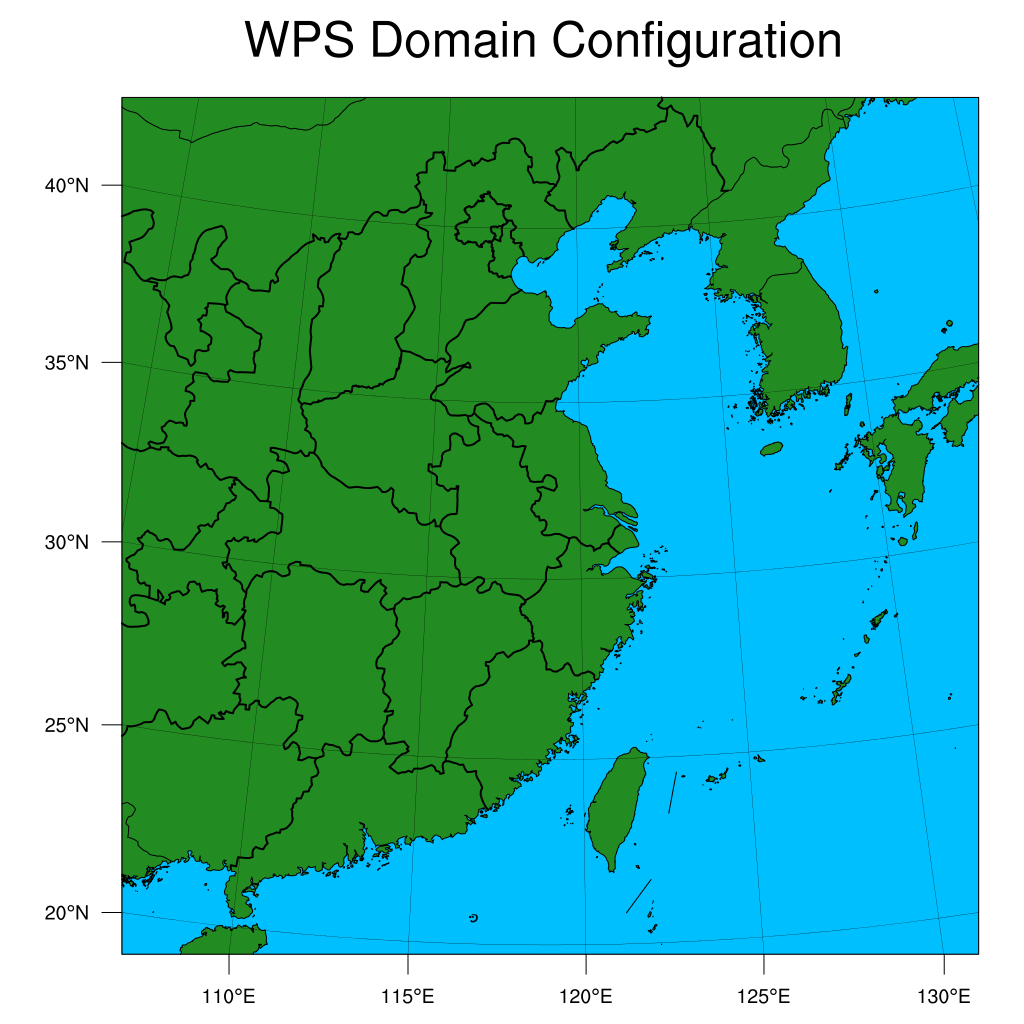
\includegraphics[trim = 15mm 5mm 5mm 24mm, clip, width=0.50\textwidth]{wps_show_dom}
    \bicaption{模拟区域}{Simulation Domain}
    \label{fig:wps_show_dom_trim}
\end{figure}

\chapter{江苏省轻污染过程数值模拟}\label{chap:evaluation}


\section{环流场形势分析}

2015年1月20日00时500hPa高空图长江中下游地区处于低压槽前,槽前受西南气流控制。21日12时槽线过境,受槽后西北气流控制。地面图上,江苏南京1月20日受低压控制,盛行风方向为低压前部偏南风控制,21日12时后受来自上游蒙古高压控制,天气条件稳定有利于污染物的累积。方向由高压前部偏北风向转为高压后部偏南风。

\begin{figure}[!htbp]
    \centering
    \begin{subfigure}[b]{0.35\textwidth}
      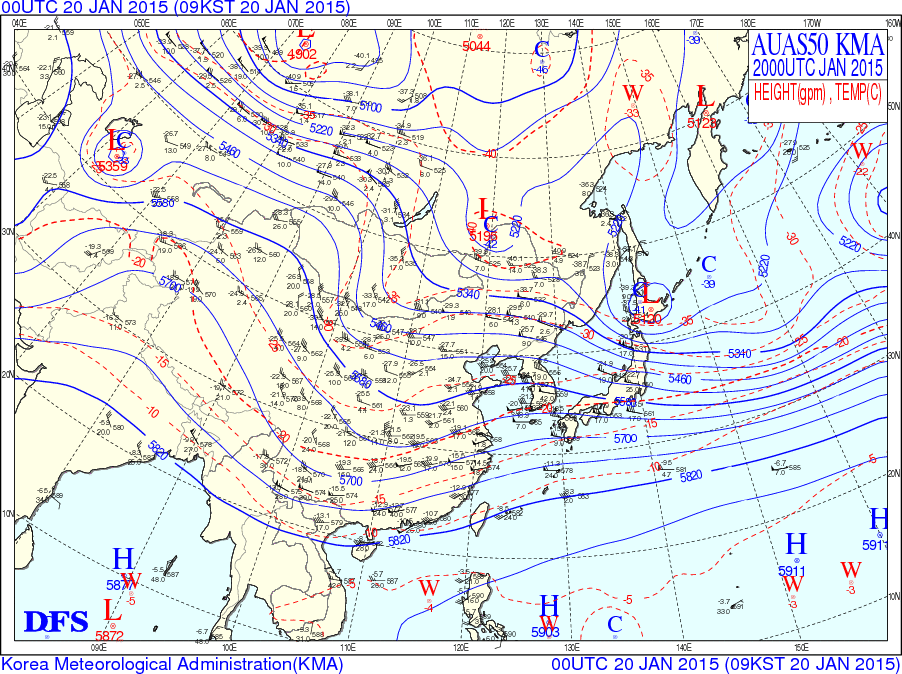
\includegraphics[width=\textwidth]{up50_2015012000}
      \caption{}
      \label{fig:up50_2015012000}
    \end{subfigure}%
    ~% add desired spacing
    \begin{subfigure}[b]{0.35\textwidth}
      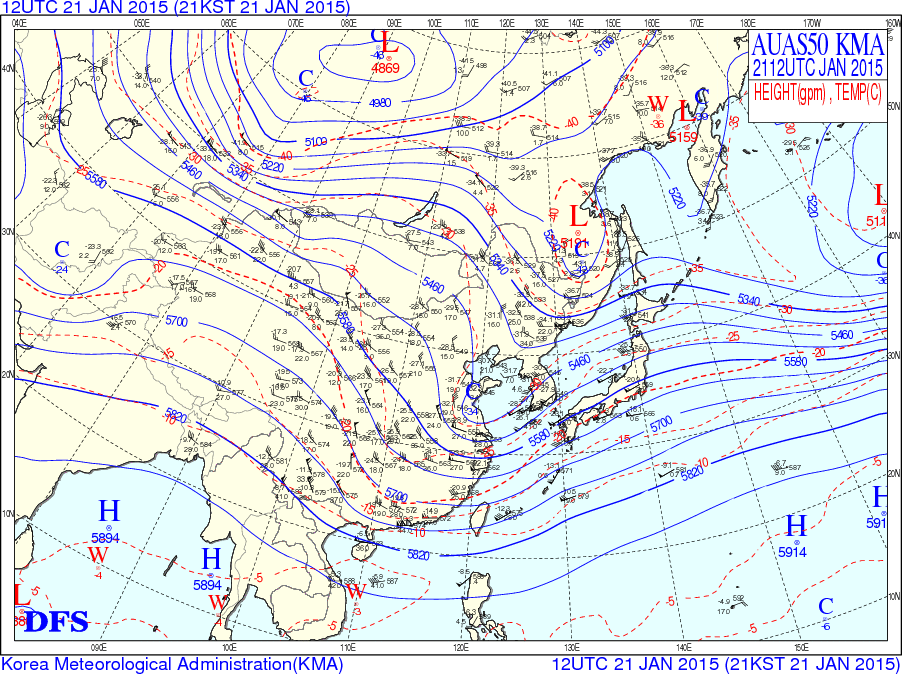
\includegraphics[width=\textwidth]{up50_2015012112}
      \caption{}
      \label{fig:up50_2015012112}
    \end{subfigure}
    \\% line break
    \begin{subfigure}[b]{0.35\textwidth}
      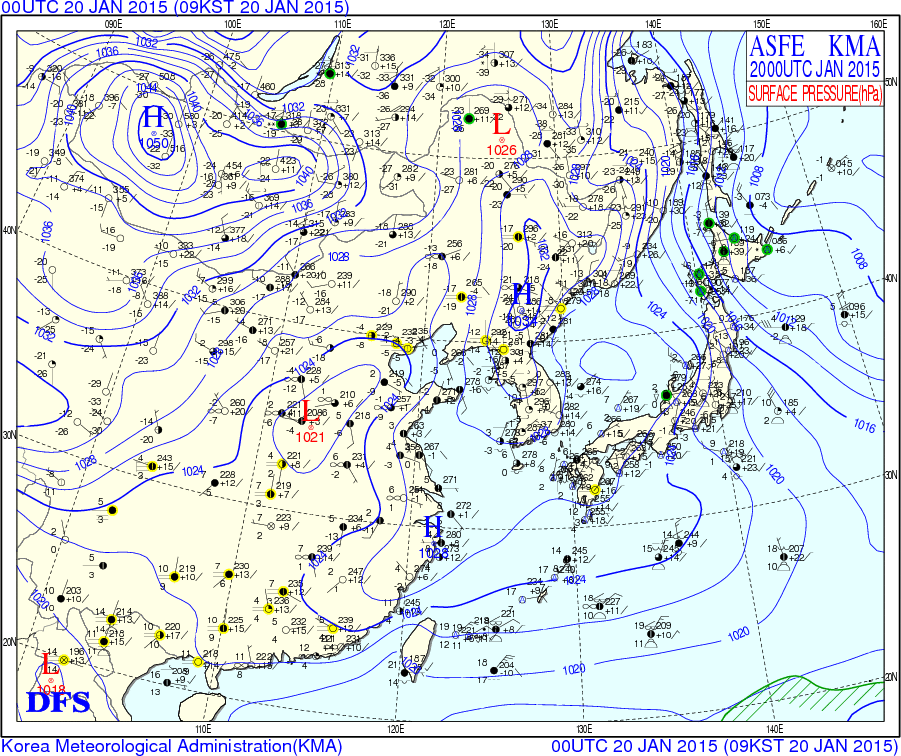
\includegraphics[width=\textwidth]{sfc3_2015012000}
      \caption{}
      \label{fig:sfc3_2015012000}
    \end{subfigure}%
    ~% add desired spacing
    \begin{subfigure}[b]{0.35\textwidth}
      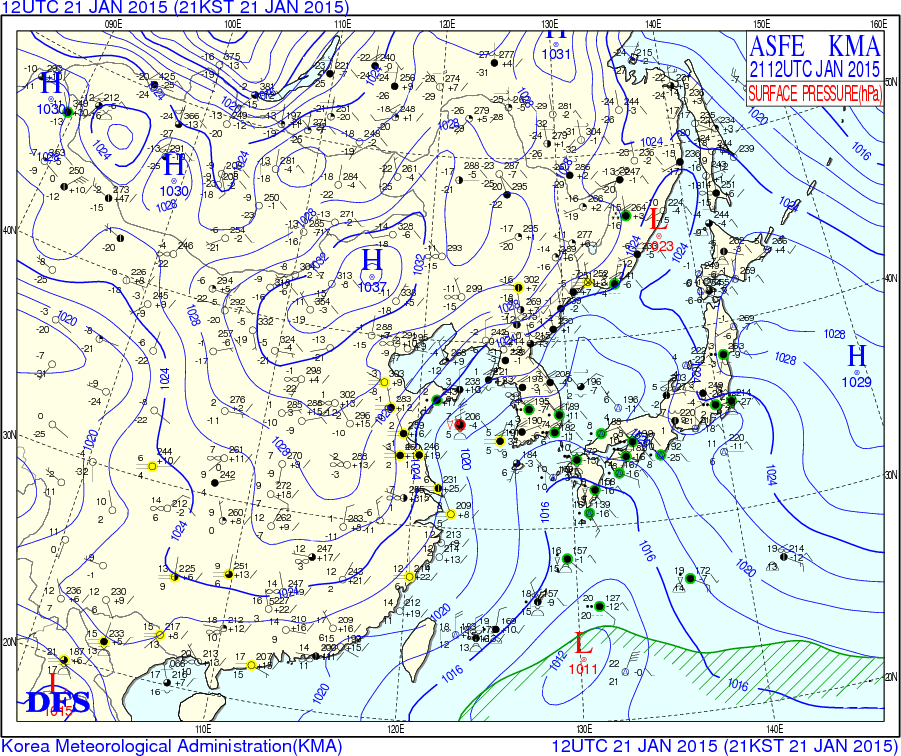
\includegraphics[width=\textwidth]{sfc3_2015012112}
      \caption{}
      \label{fig:sfc3_2015012112}
    \end{subfigure}
    \bicaption{韩国气象局天气图(a) 1月20日00时500hPa等高线图,(b) 1月21日12时500hPa等高线图,(c) 1月20日00时地面图,(d) 1月21日12时地面图。}{Korea Meteorological Administration (a) 500hPa Contour map on 00 a.m. on 20 January, (b) 500hPa Contour map on 12 a.m. on 21 January, (c) Groud map on 00 a.m. on 20 January, (d) Groud map on 12 a.m. on 21 January.}
    \label{fig:oaspl}
\end{figure}

\section{大气层结分析}

根据模拟结果选取污染过境前时刻绘制探空曲线来分析该此个例的大气层结状态,南京站在1月20日23时,探空曲线的温度露点差随高度先减少后增加,在700hPa附近存在较高湿度。大气层结存在较强垂直风切变,在一定的触发机制下有利于污染物在垂直方向的扩散,低空存在较为浅薄的逆温层且该站点的Cape能为0,层结较为稳定一定程度上有利于低层污染物堆积。

\begin{figure}[!htbp]
    \centering
    %trim option's parameter order: left bottom right top
    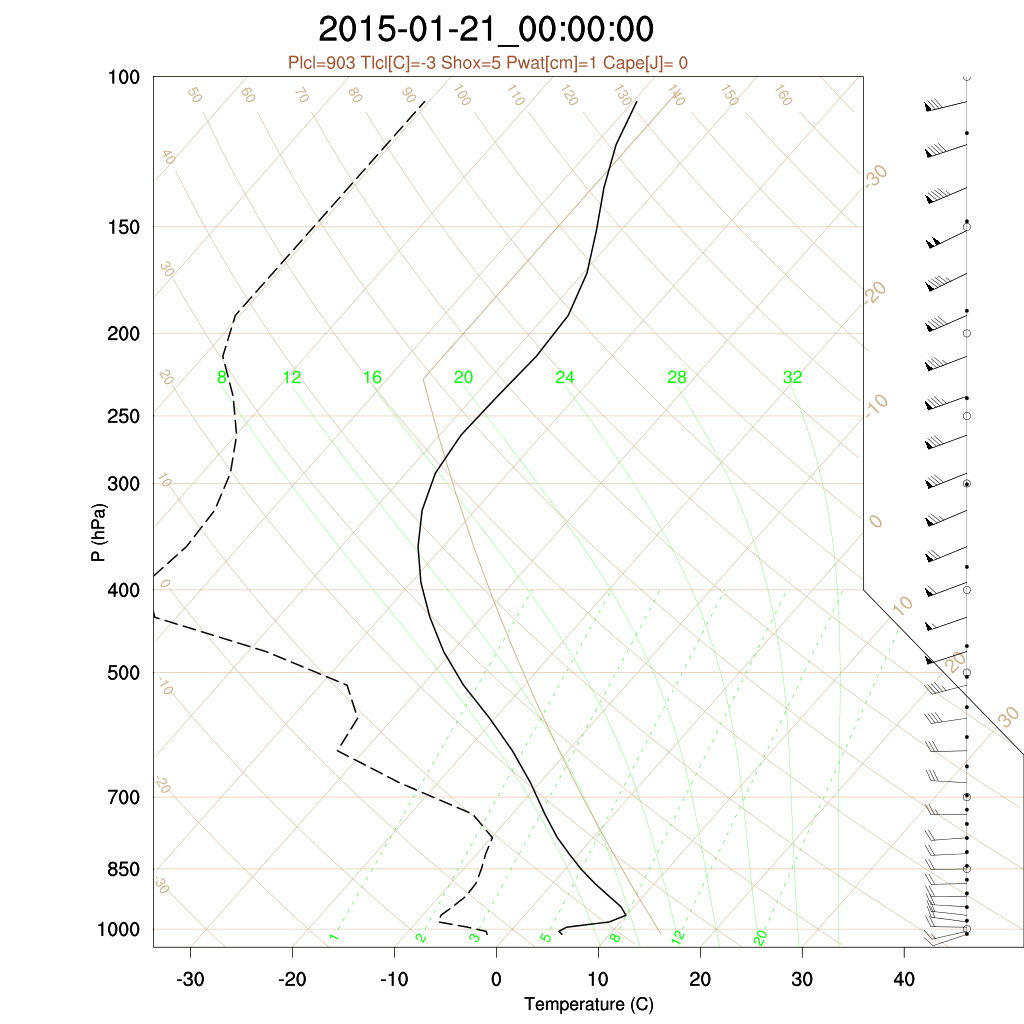
\includegraphics[trim = 5mm 0mm 0mm 0mm, clip, width=0.50\textwidth]{UW-plt_SkewT}
    \bicaption{南京站模拟的探空曲线}{Simulated sounding data curve in Nanjing station}
    \label{fig:UW-plt_SkewT_trim}
\end{figure}

\section{模拟结果评估}

通过与实况资料对比,可以发现PM25,和PM10整体浓度变化趋势一致,PM10浓度较PM25高,在22日凌晨前后模拟与观测有较大误差。CO污染物浓度较低,模拟浓度和观测浓度接近。SO2浓度也在22日同观测有所偏差,NO2和O3浓度的模拟都与实况有着较高的一致性,且误差较小。

\begin{figure}[!htbp]
    \centering
    \begin{subfigure}[b]{0.35\textwidth}
      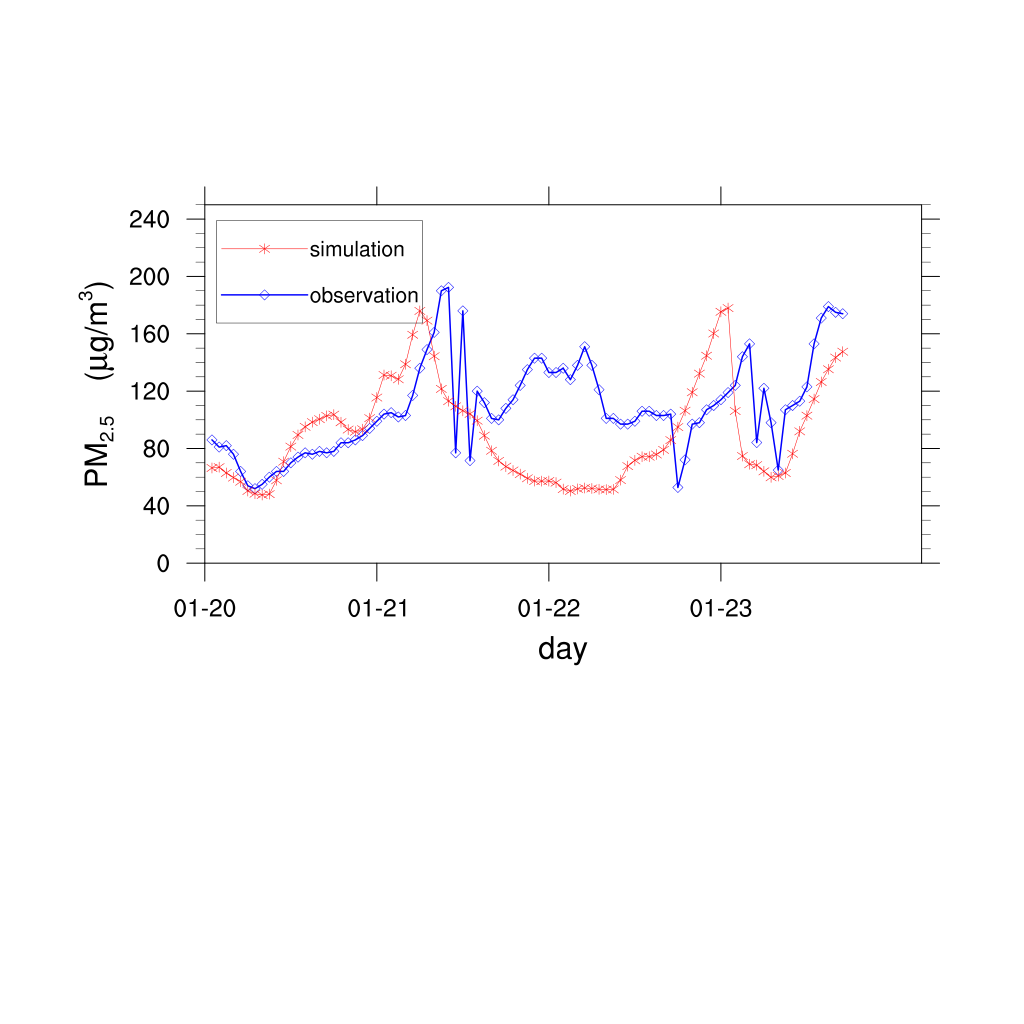
\includegraphics[trim = 20mm 120mm 30mm 50mm, clip, width=\textwidth]{plot-obe-sim-pm25}
      \caption{}
      \label{fig:plot-obe-sim-pm25}
    \end{subfigure}%
    ~% add desired spacing
    \begin{subfigure}[b]{0.35\textwidth}
      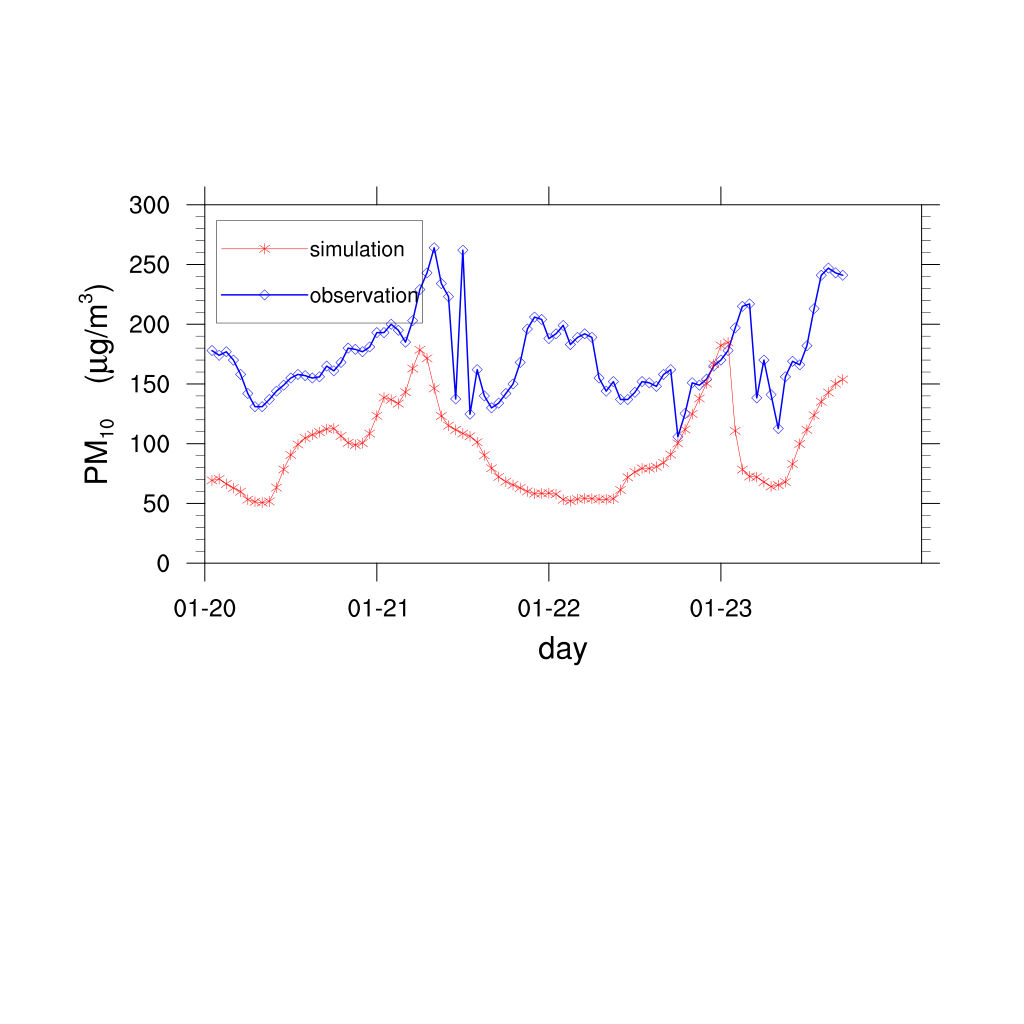
\includegraphics[trim = 20mm 120mm 30mm 50mm, clip, width=\textwidth]{plot-obe-sim-pm10}
      \caption{}
      \label{fig:plot-obe-sim-pm10}
    \end{subfigure}
    \\% line break
    \begin{subfigure}[b]{0.35\textwidth}
      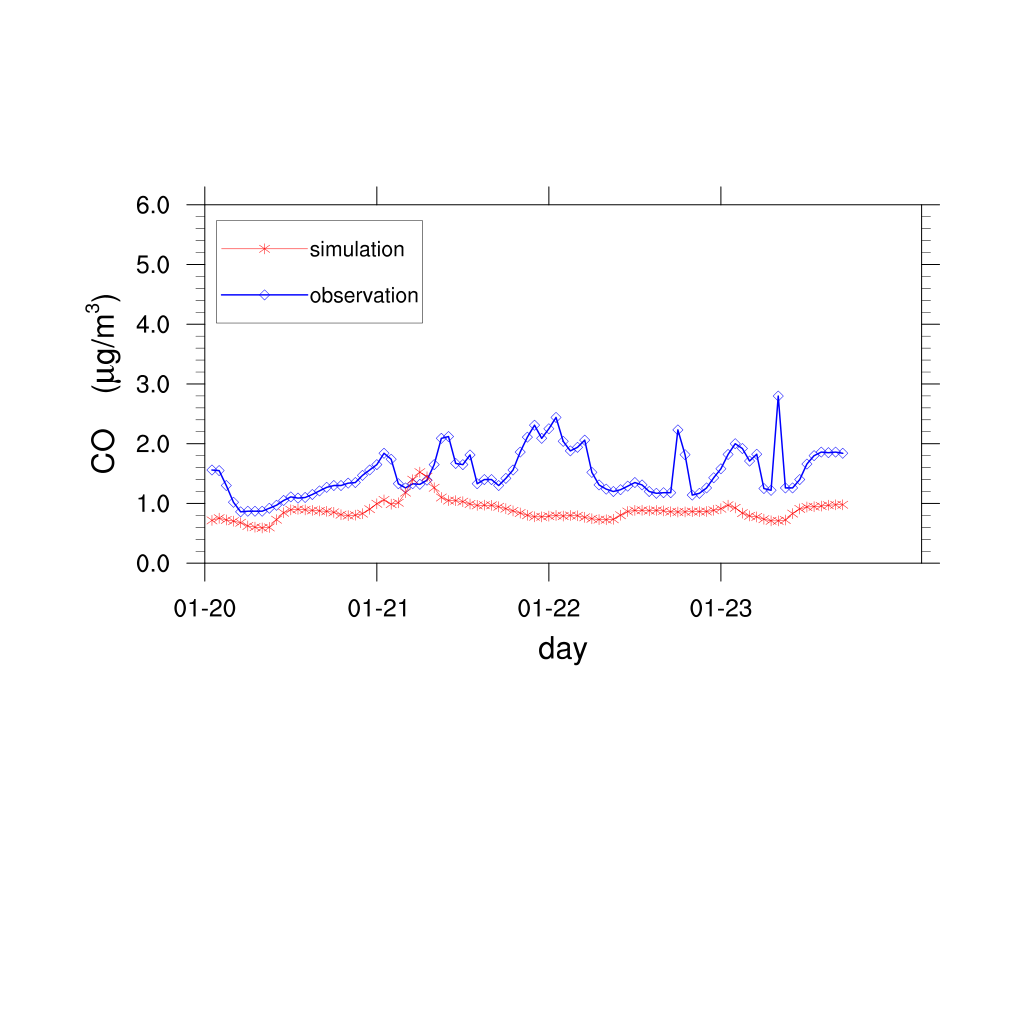
\includegraphics[trim = 20mm 120mm 30mm 50mm, clip, width=\textwidth]{plot-obe-sim-co}
      \caption{}
      \label{fig:plot-obe-sim-co}
    \end{subfigure}%
    ~% add desired spacing
    \begin{subfigure}[b]{0.35\textwidth}
      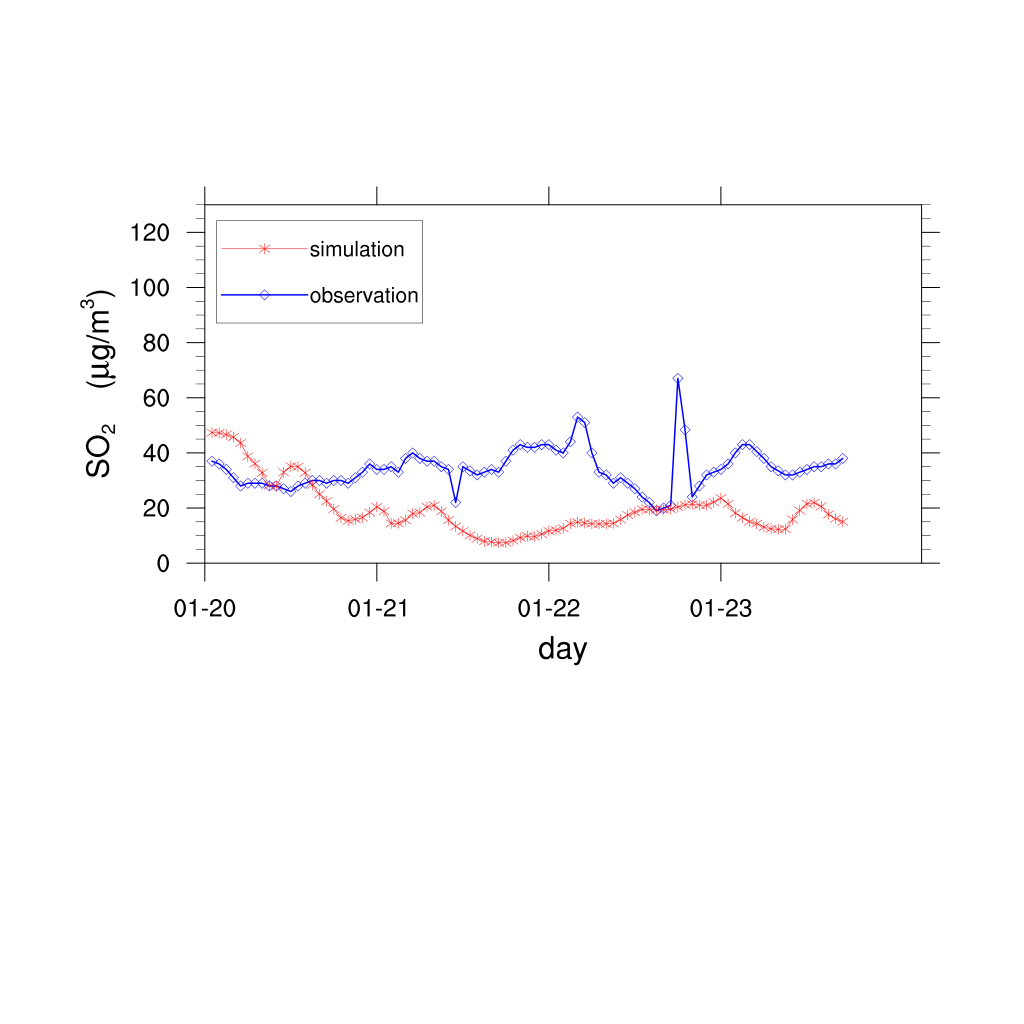
\includegraphics[trim = 20mm 120mm 30mm 50mm, clip, width=\textwidth]{plot-obe-sim-so2}
      \caption{}
      \label{fig:plot-obe-sim-so2}
    \end{subfigure}
    \begin{subfigure}[b]{0.35\textwidth}
      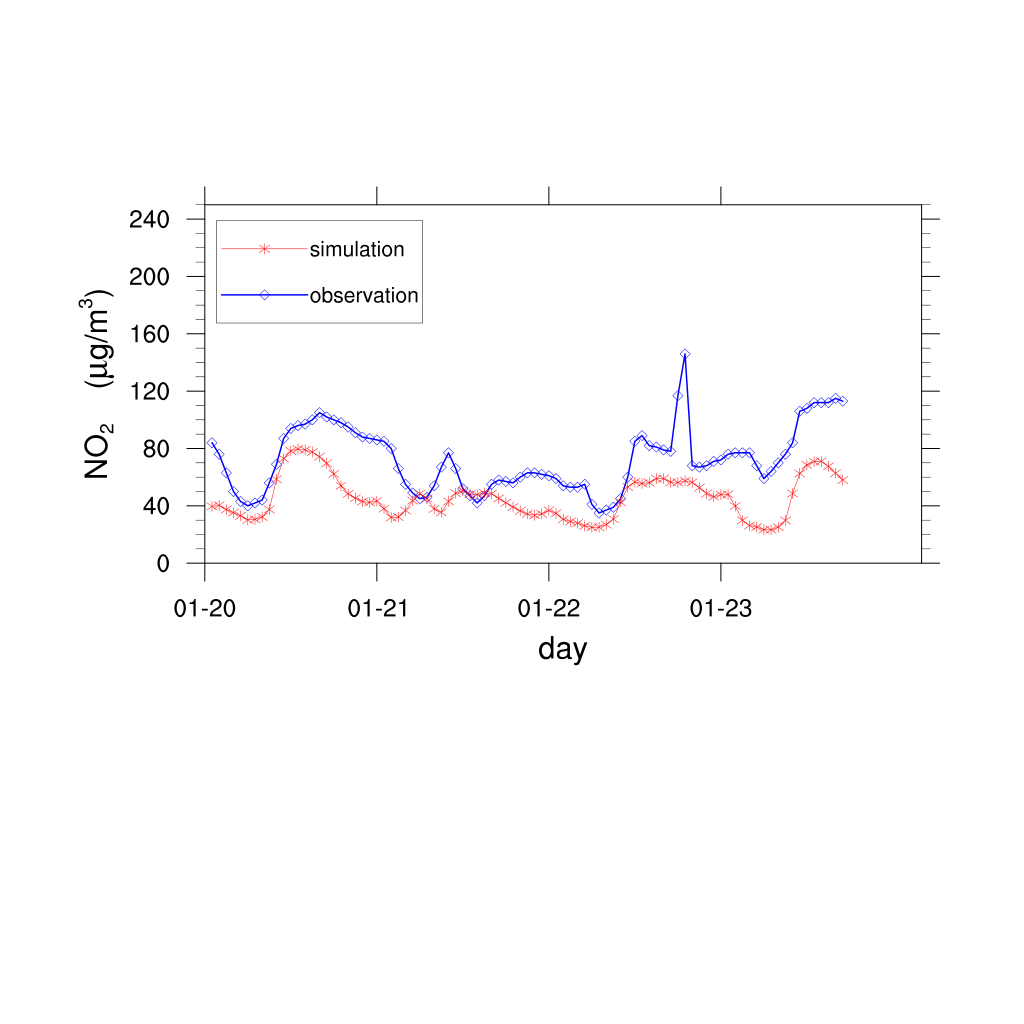
\includegraphics[trim = 20mm 120mm 30mm 50mm, clip, width=\textwidth]{plot-obe-sim-no2}
      \caption{}
      \label{fig:plot-obe-sim-no2}
    \end{subfigure}
    \begin{subfigure}[b]{0.35\textwidth}
      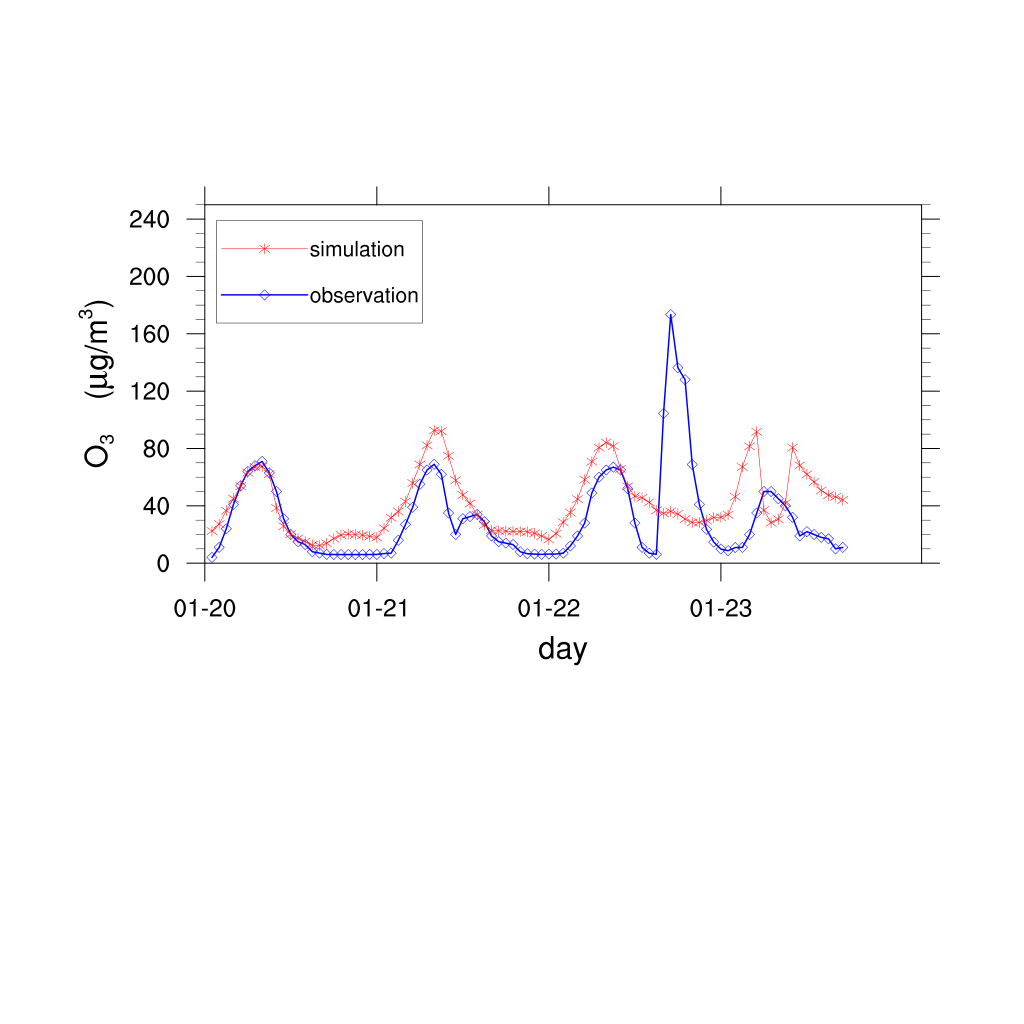
\includegraphics[trim = 20mm 120mm 30mm 50mm, clip, width=\textwidth]{plot-obe-sim-o3}
      \caption{}
      \label{fig:plot-obe-sim-o3}
    \end{subfigure}
    \bicaption{模拟与观测的污染物浓度对比 (a) PM25浓度,(b) PM10浓度,(c) CO浓度,(d) SO2浓度,(e) NO2浓度,(f) O3浓度。}{(a) The concentration of PM25, (b) The concentration of PM10, (c) The concentration of CO, (d) The concentration of SO2, (e) The concentration of NO2, (f) The concentration of O3.}
    \label{fig:oaspl}
\end{figure}

\section{边界层与污染物浓度关系}

随着白天温度的上升,热力对流作用占据对流的主导地位,大多数污染物都在对流扩散稀释的作用下,随着边界层的高度增加,其浓度均有所下降,呈现负相关。对流层臭氧却与边界层高度呈现正相关,主要原因是由于,臭氧的生成需要光照和热量,对流边界层的高度白天大于夜间,也受热力影响,因而在午后臭氧的浓度均达到峰值,同时可以从图中可以发现臭氧的峰值变化相交边界层高度更具有周期性,由此臭氧对日变化更具敏感性。

\begin{figure}[!htbp]
    \centering
    \begin{subfigure}[b]{0.35\textwidth}
      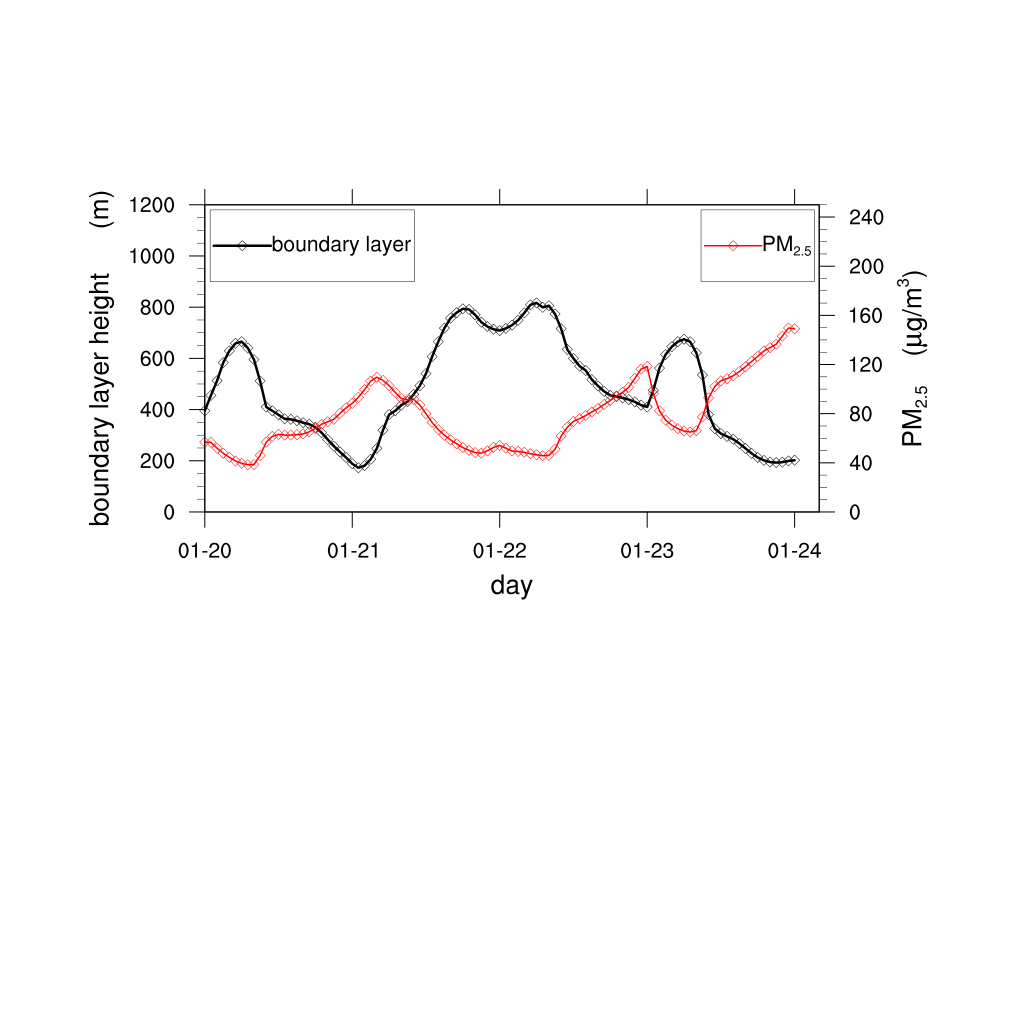
\includegraphics[trim = 20mm 120mm 30mm 50mm, clip, width=\textwidth]{bjl_pm25}
      \caption{}
      \label{fig:bjl_pm25}
    \end{subfigure}%
    ~% add desired spacing
    \begin{subfigure}[b]{0.35\textwidth}
      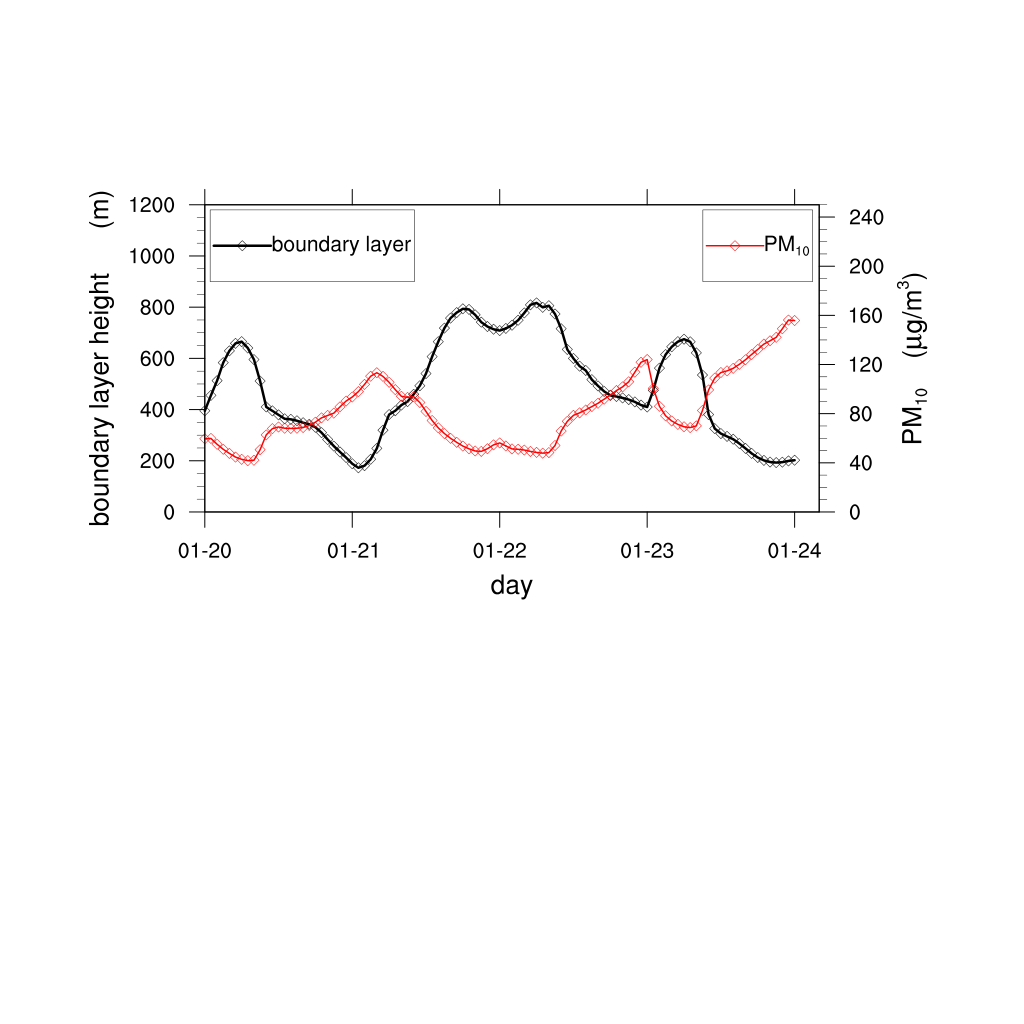
\includegraphics[trim = 20mm 120mm 30mm 50mm, clip, width=\textwidth]{bjl_pm10}
      \caption{}
			\label{fig:bjl_pm10}
    \end{subfigure}
    \\% line break
    \begin{subfigure}[b]{0.35\textwidth}
      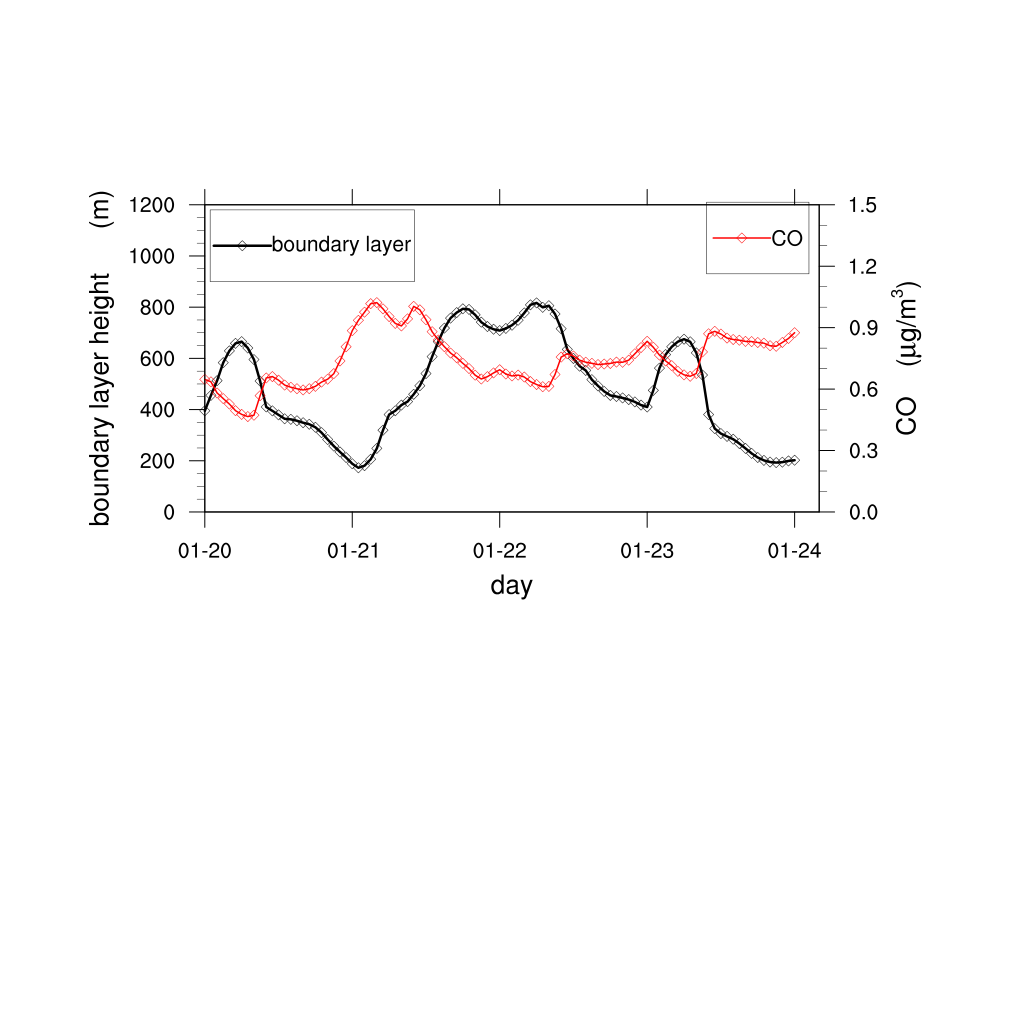
\includegraphics[trim = 20mm 120mm 30mm 50mm, clip, width=\textwidth]{bjl_co}
      \caption{}
			\label{fig:bjl_co}
    \end{subfigure}%
    ~% add desired spacing
    \begin{subfigure}[b]{0.35\textwidth}
      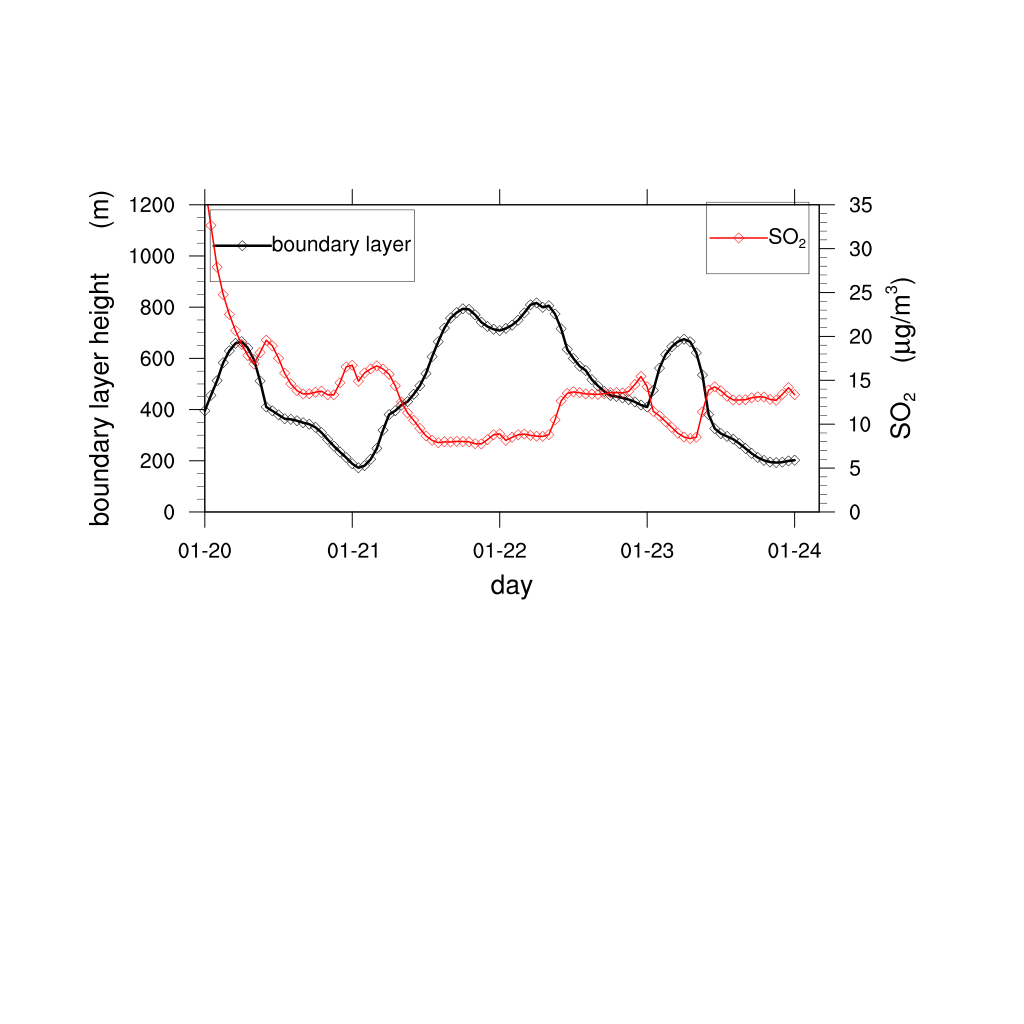
\includegraphics[trim = 20mm 120mm 30mm 50mm, clip, width=\textwidth]{bjl_so2}
      \caption{}
			\label{fig:bjl_so2}
    \end{subfigure}
    \begin{subfigure}[b]{0.35\textwidth}
      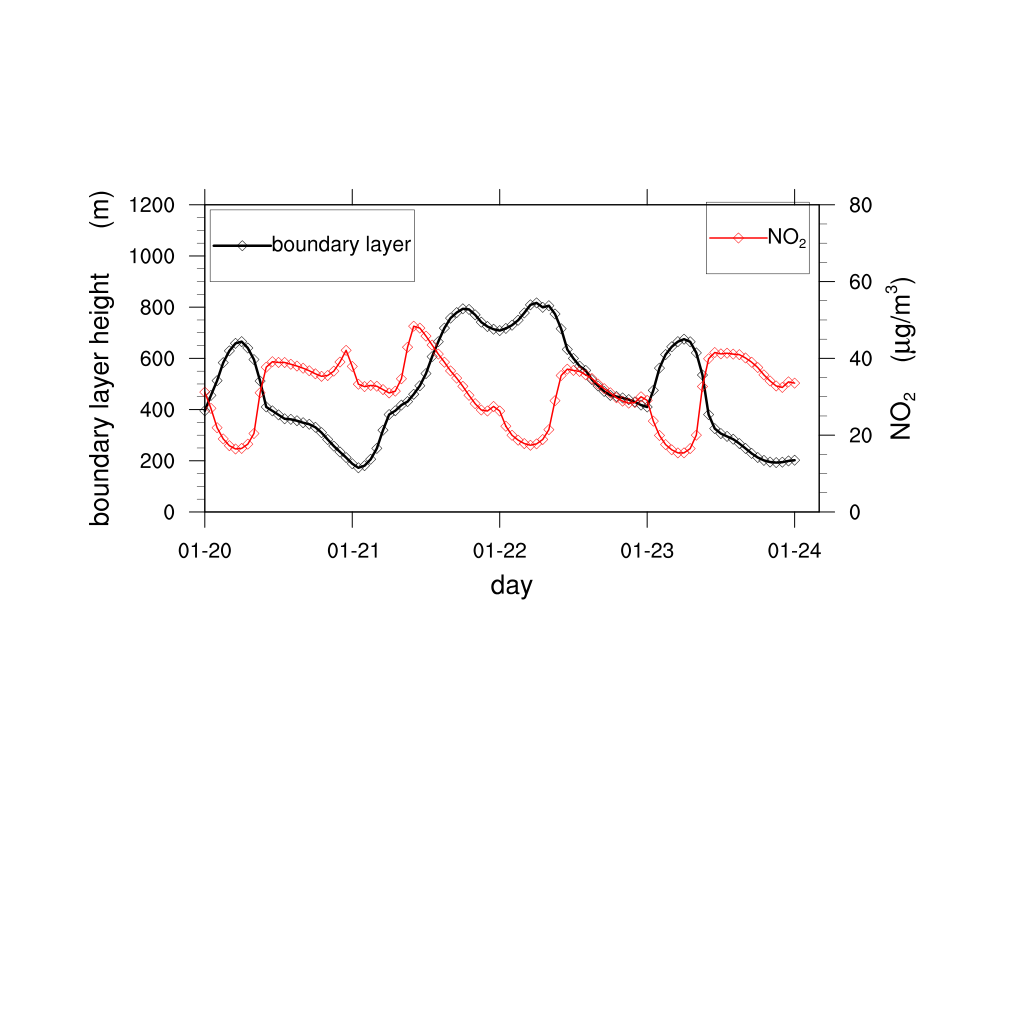
\includegraphics[trim = 20mm 120mm 30mm 50mm, clip, width=\textwidth]{bjl_no2}
      \caption{}
			\label{fig:bjl_no2}
    \end{subfigure}
    \begin{subfigure}[b]{0.35\textwidth}
      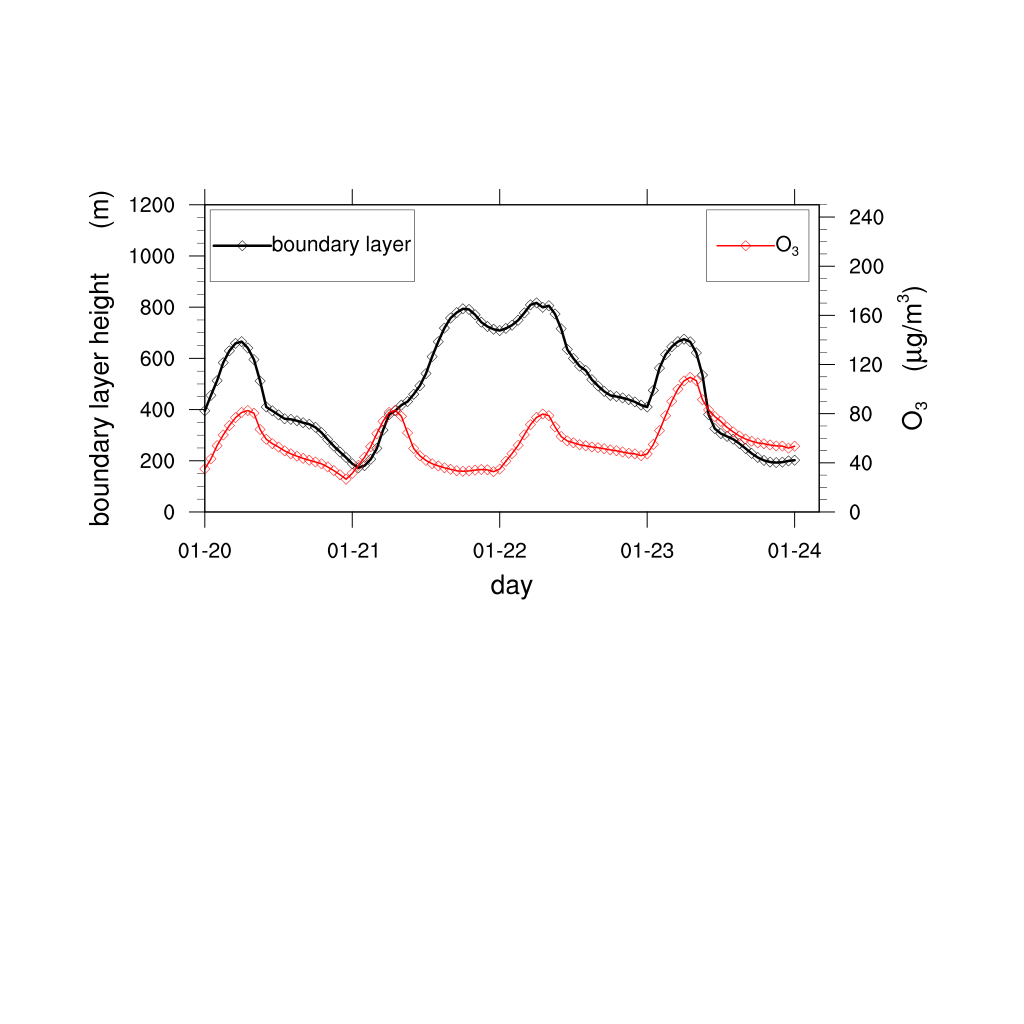
\includegraphics[trim = 20mm 120mm 30mm 50mm, clip, width=\textwidth]{bjl_o3}
      \caption{}
			\label{fig:bjl_o3}
    \end{subfigure}
		\bicaption{边界层高度与污染物浓度对比 (a) PM25浓度,(b) PM10浓度,(c) CO浓度, (d) SO2浓度, (e) NO2浓度,(f) O3浓度。}{Comparison between Boundary layer height and pollution concentration (a) The concentration of PM25, (b) The concentration of PM10, (c) The concentration of CO, (d) The concentration of SO2, (e) The concentration of NO2, (f) The concentration of O3.}
    \label{fig:oaspl}
\end{figure}

